% Change to use the correct class file for your paper.
\documentclass[10pt]{report}
%\nocopyrightspacetrue

%\pagenumbering{arabic}

\usepackage{amsfonts}
\usepackage{array}
\usepackage{booktabs}
\usepackage{color}
\usepackage{colortbl}
\usepackage{endnotes}
%\usepackage[cm]{fullpage}
\usepackage[margin=0.5in]{geometry}
\usepackage{graphicx}    % For importing graphics
\usepackage[draft]{hyperref}    % Creates hyperlinks from ref/cite 
%\usepackage{hyperref}    % Creates hyperlinks from ref/cite 
\usepackage{multirow}
\hypersetup{pdfstartview=FitH}
%\usepackage{subfig}
\usepackage{subfigure}
\usepackage{tabularx}
\usepackage{url}         %
\usepackage{xspace}
%\usepackage[bf,skip=5pt]{caption}
\usepackage[skip=5pt]{caption}
\usepackage{comment}
\usepackage{amssymb}
\usepackage{amsmath}
\usepackage{amsfonts}
\usepackage{wrapfig}

%\usepackage{xcolor}
\usepackage{colortbl}
\usepackage{threeparttable}

\DeclareCaptionType{copyrightbox}

\newlength\SUBSIZE

\renewcommand{\arraystretch}{1.2} % Space out rows in tables

\newcommand{\projname}{Super Super Sweet (S$^3$) Project Name\xspace}
\newcommand{\ra}{$\rightarrow$\xspace}

\setlength\paperheight {11in}
\setlength\paperwidth {8.5in}

% Set the graphics path
\graphicspath{{../figs/}{../images/build/}}
%\DeclareGraphicsExtensions{.pdf,.png,.jpg}


% No space between bibliography items:
\let\oldthebibliography=\thebibliography
  \let\endoldthebibliography=\endthebibliography
  \renewenvironment{thebibliography}[1]{%
    \begin{oldthebibliography}{#1}%
      \setlength{\parskip}{0ex}%
      \setlength{\itemsep}{0ex}%
  }%
  {%
    \end{oldthebibliography}%
  }
\setlength{\parindent}{5mm}

\newcommand{\sdr}{$\mu$SDR\xspace}
\newcommand{\realtilde}{\raise.17ex\hbox{$\scriptstyle\sim$}}

\begin{document}

%\CopyrightYear{} 
%\crdata{}
\clubpenalty=10000 
\widowpenalty = 10000

%\title{A Compact, Inexpensive, and Battery-Powered\\
%  Software-Defined Radio Platform}
%\title{Reconfiguring the Software-Defined Radio\\to Improve Power,
%  Price, and Proportions}
\title{SDR notes}

\author{Ye-sheng Kuo}
\date{May 2012}
\maketitle

\chapter{Demodulation of 802.15.4}
\section{Demodulation equation}
The receiver uses the following equation to demodulate the signal.
\begin{equation}
d(t) = R_Q(t)\times R_I(t-\tau) - R_Q(t-\tau)\times R_I(t)
\end{equation}

where the $R_I(t)/R_Q(t)$ are received In-phase/Quad-phase signals, $\tau$ is the sampling period. Bit decoding depends on
the sign of $d(t)$. If $d(t)>0$, the decoded bit equals 1 and vice versa.

\section{Decoding principle}
The 802.15.4 standard uses OQPSK modulation. The In-phase and Quad-phase are shifted by 1/2 symbol time. The symbol time 
is 1/2 period of sine wave. Namely, the In-phase and Quad-phase are shifted by 1/4 period of sine wave. Thus, the In-phase
and Quad-phase can be expressed as $\pm sin(t + \theta)$ and $\pm cos(t + \theta)$. Where $\theta \in \{0, \tfrac{\pi}{2}\}$.

For example, one combination of In-phase/Quad-phase is $cos(t)$ and $sin(t), 0<t<\tfrac{pi}{2}$. By applying the demodulation
equation,
\begin{align}
d(t)&= sin(t)\times cos(t-\tau) - sin(t-\tau)\times cos(t) \\
d(t)&= sin(t)\left[cos(t)cos(\tau) + sin(t)sin(\tau)\right] - cos(t)\left[sin(t)cos(\tau) - cos(t)sin(\tau)\right] \\
d(t)&= sin^2(t)sin(\tau) + cos^2(t)sin(\tau) = sin(\tau)
\end{align}
Therefore, $d(t)$ depends on the sampleing period only. In this example, $d(t)$ is greater than 0 and remains constant 
during the half-symbol period. The following table lists the total combination of I/Q signals.

\begin{table}[h!]
\centering
	\begin{tabular}{|c|c|c|}
		\hline
		In-phase & Quad-phase 	& decoded equation \\ \hline	
		$cos(t)$ & $sin(t)$		& $sin(\tau)$\\ \hline
		$cos(t)$ & $-sin(t)$	& $-sin(\tau)$\\ \hline
		$-cos(t)$ & $sin(t)$	& $-sin(\tau)$\\ \hline
		$-cos(t)$ & $-sin(t)$	& $sin(\tau)$\\ \hline
		$sin(t)$ & $cos(t)$		& $-sin(\tau)$\\ \hline
		$sin(t)$ & $-cos(t)$	& $sin(\tau)$\\ \hline
		$-sin(t)$ & $cos(t)$	& $sin(\tau)$\\ \hline
		$-sin(t)$ & $-cos(t)$	& $-sin(\tau)$\\ \hline
	\end{tabular}
	\label{tab:demux}
	\caption{}
\end{table}

Therefore, the receiver simply determines the incoming bit from the sign of $d(t)$. Note that the I/Q signals coming
at the symbol rate of 1$\mu$s, and the I/Q shift by 0.5$\mu$s. Every 0.5$\mu$s generates a bit. Bit rate is 2MHz and 
half-byte is mapped to 32 bits chip sequence, which is 16$\mu$s.

\chapter{Frequency Mismatch}
\section{Carrier frequency mismatch in single TX/RX}
Considering the transmitted In-phase signal $S_I(t)$, Quad-phase signal $S_Q(t)$ and the carrier frequency of
transmitter $f_{c1}$. The transmitted signal can be writted as $S(t)$

\begin{equation}
S(t) = S_I(t) \times cos(2\pi \times f_{c1} \times t ) + S_Q(t) \times sin(2\pi \times f_{c1} \times f)
\end{equation}

Ignoring the channel characteristic and absense of noice, the received signal $R(t) = S(t)$. If there is a
mismatch in carrier frequency, the receiver carrier frequency $f_{c2} \neq f_{c1}$. The received In-phase signal
can be expressed as \\
$r_I(t) = R(t) \times cos(2\pi \times f_{c2} \times t)$.

\begin{eqnarray}
r_I(t) = \left[S_I(t) \times cos(\omega_{c1}t) + S_Q(t) \times sin(\omega_{c1}t)\right] \times cos(\omega_{c2}t) \\
r_I(t) = S_I(t) \times cos(\omega_{c1}t) \times cos(\omega_{c2}t) + S_Q(t) \times sin(\omega_{c1}t) \times cos(\omega_{c2}t)
\end{eqnarray}

Where $\omega_{c1,2} = 2\pi\times f_{c1,2}$. Simplifying the equation by product to sum identities.
\begin{equation}
r_I(t) = 
\tfrac{1}{2}S_I(t)\left[cos((\omega_{c1}-\omega_{c2})t) + cos((\omega_{c1}+\omega_{c2})t)\right] + 
\tfrac{1}{2}S_Q(t)\left[sin((\omega_{c1}-\omega_{c2})t) + sin((\omega_{c1}+\omega_{c2})t)\right]
\end{equation}

By removing high frequency components ($\omega_{c1}+\omega_{c2}$). In-phase baseband signal $r_{IB}(t)$ can be expressed
\begin{equation}
r_{IB}(t) = \tfrac{1}{2}S_I(t)\times cos(\Delta\omega t) - \tfrac{1}{2}S_Q(t)\times sin(\Delta\omega t)
\end{equation}

Similarly, Quad-phase baseband signal $r_{QB}(t)$
\begin{equation}
r_{QB}(t) = \tfrac{1}{2}S_I(t)\times sin(\Delta\omega t) + \tfrac{1}{2}S_Q(t)\times cos(\Delta\omega t)
\end{equation}

where $\Delta\omega = \omega_{c2} - \omega_{c1}$. By Rearranging these queations, we can express the
following.
\[
\begin{bmatrix}
	r_{IB}(t) \\
	r_{QB}(t) 
\end{bmatrix}
=
\begin{bmatrix}
	cos(\Delta\omega t) & -sin(\Delta\omega t) \\
	sin(\Delta\omega t) & cos(\Delta\omega t)
\end{bmatrix}
\times
\begin{bmatrix}
	{}^1/_2\cdot S_I(t)\\
	{}^1/_2\cdot S_Q(t)\\
\end{bmatrix}
\]
We can clearly see that the frequency mismatch is equivalent to the rotation 
of complex coordinate with angular velocity $\Delta\omega$. Hense, by 
measuring the rotation speed and direction, we can back calculate the 
frequency offset between receiver and transmitter. In the O-QPSK modulation, 
I/Q signal at any given time map to a unit circle on constellation. 
Measuring both clockwise and counter clockwise rotation angle at fixed 
interval tells the receiver's carrier frequency is leading or legging. 
With this information, radio is able to self-compensate the frequency 
mismatch and we called it \textit{Automatic Frequency Compensation} or AFC. 

\begin{table}
	\centering
	\begin{tabular}{|c|c|c|} \hline
		\rowcolor[gray]{0}
		  {\sc {\color{white} AGC mode}}
		& {\sc {\color{white} AFC mode}}
		& {\sc {\color{white} ARR}}
		\\ \hline
		SFD-latch 	& Enable 	& 93.3\%	\\ \hline
		Continuous	& Enable	& 95.5\%	\\ \hline
		SFD-latch 	& Disable	& 94.5\%	\\ \hline
		Continuous	& Disable	& 95.1\%	\\ \hline
	\end{tabular}
    \caption{Acknowledgment reception rate (ARR) for two constructively
interfering transmitters with respect to different AGC modes and AFC mode. 
We transmitted 10,000 ACKs per transmitter per experiment. With AFC disable,
carrier frequencies of TX and RX is off by 16.4KHz. In both case of AFC mode,
continuous AGC works better. Enabling the AFC worsen the reception rate for
SFD-Latch AGC simply because the baseband signal is attenuated by low-frequency
envelope.}
	\label{tab:ARR_versus_agc_afc_mode}
\end{table}

From table ~\ref{tab:ARR_versus_agc_afc_mode}, data shows that the ARR decrease
in SFD-Latch type AGC when AFC is enabled. Since the AFC tries to sompensate the
frequency difference between TX and RX, the duration of local minimum becomes
larger whereas no significant change on Continuous AGC mode. Continuous AGC with
AFC could potentially increase the reception rate in longer identical packet 
collision.

\subsection{Automatic Frequency Compensation}
The 802.15.4 uses O-QOSK modulation. At any given of time, the in-phase and quad-phase
have only 8 combinations which is listed in table~\ref{tab:demux}. The key concept 
is that the in-phase and quad-phase signal vector is always on the unit circle of 
complex plane. Moreover, the signal vector is always rotating at angular velocity
$\omega = \tfrac{\pi/2}{0.5 \mu s}$. However, if the frequency of transmitter
and receiver doesn't match, the angular velocities toward clockwise and counter-clockwise
are different. Thus, by sampling the vector at constant rate and calculate angle difference
toward two different direction, we are able to tell the frequency is leading or lagging.
In usdr, we implemented a simple cordic core to measure the angle of input vector with
sampling rate $= 250 Ksps$. The delta angle should be $\pm\pi/4$ if frequencies are perfectly
matched. By comparing the delta angle with $\pm\pi/4$, radio is able to self-align
its carrier frequency to the incoming packet.
\begin{figure}[h]
\centering
	\includegraphics[width=0.6\columnwidth]{frequency_compensate/freq_compensate}
	\caption{}
	\label{fig:afc_freq_error}
\end{figure}

Figure~\ref{fig:afc_freq_error} shows capability of AFC to correct the frequency 
mismatch. The original frequency mismatch is set to be 50 KHz. The figure shows how
much frequency mismatch after automatic frequency compensation within a packet length.
In these simulations, the packet lengths are set to be 127 and 64 bytes. The frequency  
step size in both simulation is 300 Hz. Thus, if the RMS frequency error $<$ 300 Hz, 
the AFC successfully compensated all frequency mismatch. We can clearly see that 
for larger SNR, AFC works better. In addition, more opportunities to compensate the
frequency in longer packet. Hence, frequency error is smaller in 127 bytes packet.


\subsection{Demodulation with frequency mismatch}
\label{1tx1rx_mismatch}
Recall the demodulation equation $d(t) = S_Q(t)\times S_I(t-\tau) - S_Q(t-\tau)\times S_I(t)$.
Under the frequency mismatch scenario, the recieved $r_{IB}(t)$ and $r_{QB}(t)$ can be substituded by $S_I(t)$ and $S_Q(t)$. 
$d_f(t)$ can be written in following:
\begin{align}
d_f(t) = &
\left[-\tfrac{1}{2}S_I(t)sin(\Delta\omega t)+\tfrac{1}{2}S_Q(t)cos(\Delta\omega t)\right] \times
\left[\tfrac{1}{2}S_I(t-\tau)cos(\Delta\omega(t-\tau))+\tfrac{1}{2}S_Q(t-\tau)sin(\Delta\omega(t-\tau))\right] \nonumber \\
&  -\left[-\tfrac{1}{2}S_I(t-\tau)sin(\Delta\omega(t-\tau))+\tfrac{1}{2}S_Q(t-\tau)cos(\Delta\omega(t-\tau))\right] \times
\left[\tfrac{1}{2}S_I(t)cos(\Delta\omega t) + \tfrac{1}{2}S_Q(t)sin(\Delta\omega t)\right]
\end{align}

Assuming that the $\Delta\omega\times\tau$ is small enough.
\begin{align}
cos(\Delta\omega(t-\tau))& \approx cos(\Delta\omega t) \\
sin(\Delta\omega(t-\tau))& \approx sin(\Delta\omega t)
\end{align}

The equation can be further simplified.
\begin{align}
d_f(t) \approx &
\left[-\tfrac{1}{2}S_I(t)sin(\Delta\omega t)+\tfrac{1}{2}S_Q(t)cos(\Delta\omega t)\right] \times
\left[\tfrac{1}{2}S_I(t-\tau)cos(\Delta\omega t)+\tfrac{1}{2}S_Q(t-\tau)sin(\Delta\omega t)\right] \nonumber \\
& -\left[-\tfrac{1}{2}S_I(t-\tau)sin(\Delta\omega t)+\tfrac{1}{2}S_Q(t-\tau)cos(\Delta\omega t)\right] \times
\left[\tfrac{1}{2}S_I(t)cos(\Delta\omega t) + \tfrac{1}{2}S_Q(t)sin(\Delta\omega t)\right]\\
\approx & \left[-\tfrac{1}{4}S_I(t)S_Q(t-\tau)sin^2(\Delta\omega t) + \tfrac{1}{4}S_I(t-\tau)S_Q(t)cos^2(\Delta\omega t)\right]\nonumber\\
& -\left[\tfrac{1}{4}S_I(t)S_Q(t-\tau)cos^2(\Delta\omega t) -\tfrac{1}{4}S_I(t-\tau)S_Q(t)sin^2(\Delta\omega t)\right]\\
\approx &\tfrac{1}{2}\left[S_Q(t)S_I(t-\tau) - S_Q(t-\tau)S_I(t)\right]
\end{align}

The decoded equation $d_f(t)$ is linear scaling of $d(t)$. The sign of $d_f(t)$ and $d(t)$ are identical. Therefore, 
the decoder scheme still function if there is a mismatch between transmitter and receiver.


\clearpage
\section{Carrier frequency mismatch in double TX, single RX}
\label{sec:2tx1rx}
In this scenario, two TX node transmit the identical baseband signal simultaneously. Assuming the TX nodes have different
carrier frequency $f_{c1}$ and $f_{c2}$, and receiver's frequency is $f_{cr}$. We simply assume that $R(t) = S(t)$.
\begin{equation}
R(t) = S(t) = S_I(t)\left[cos(\omega_{c1}t) + cos(\omega_{c2}t)\right] + S_Q(t)\left[sin(\omega_{c1}t) + sin(\omega_{c2}t)\right]
\end{equation}

Simplifying the equation by sum-to-product identities.
\begin{align}
R(t)& = S_I(t)\left[2cos(\tfrac{\omega_{c1}+\omega_{c2}}{2}t)cos(\tfrac{\omega_{c1}-\omega_{c2}}{2}t)\right] +
S_Q(t)\left[2sin(\tfrac{\omega_{c1}+\omega_{c2}}{2}t)cos(\tfrac{\omega_{c1}-\omega_{c2}}{2}t)\right] \\
& = cos(\tfrac{\omega_{c1}-\omega_{c2}}{2}t)\left[
2S_I(t)cos(\tfrac{\omega_{c1}+\omega_{c2}}{2}t) + 2S_Q(t)sin(\tfrac{\omega_{c1}+\omega_{c2}}{2}t) \right]
\end{align}

The received In-phase signal $r_I(t)$ can be expressed as following:
\begin{equation}
r_I(t) = R(t) \times cos(\omega_{cr}t) \\
\end{equation}
\begin{align}
r_I(t) =  cos(\tfrac{\omega_{c1}-\omega_{c2}}{2}t)\{
&S_I(t)\left[cos(\tfrac{\omega_{c1}+\omega_{c2}-2\omega_{cr}}{2}t) + cos(\tfrac{\omega_{c1}+\omega_{c2}+2\omega_{cr}}{2}t)\right] + \nonumber \\
&S_Q(t)\left[sin(\tfrac{\omega_{c1}+\omega_{c2}-2\omega_{cr}}{2}t) + sin(\tfrac{\omega_{c1}+\omega_{c2}+2\omega_{cr}}{2}t)\right] 
\}
\end{align}

Let $\Delta\omega_1 = (\omega_{c1} - \omega_{cr})$ and $\Delta\omega_2 = (\omega_{c2} - \omega_{cr})$. By removing 
high frequency tems, $r_{IB}(t)$ can be simplified.
\begin{equation}
r_{IB}(t) = cos(\tfrac{\Delta\omega_1-\Delta\omega_2}{2}t)\left[
S_I(t)cos(\tfrac{\Delta\omega_1+\Delta\omega_2}{2}t) + S_Q(t)sin(\tfrac{\Delta\omega_1+\Delta\omega_2}{2}t)\right]
\end{equation}

Similarily, the received Quad-phase baseband signal $r_{QB}(t)$ can be derived from $R(t)\times sin(\omega_{cr}t)$.
\begin{equation}
r_{QB}(t) = cos(\tfrac{\Delta\omega_1-\Delta\omega_2}{2}t)\left[
-S_I(t)sin(\tfrac{\Delta\omega_1+\Delta\omega_2}{2}t) + S_Q(t)cos(\tfrac{\Delta\omega_1+\Delta\omega_2}{2}t)\right]
\end{equation}

From section~\ref{1tx1rx_mismatch}, we can conclude that if $(\Delta\omega_1-\Delta\omega_2)t$ is small enough, the 
decoding equation just simply scaling by $cos^2((\Delta\omega_1-\Delta\omega_2)t)$, which is always greater than zero. 
The sign of decoding equation remains the same as no frequency mismatch.

\section{Envelop Modeling}
\subsection{Theoretical Method}
\label{sec:envelop_modeling}
Considering a simplified model, there are two transmitters and one receiver with their carrier frequency 
$f_{c1}$, $f_{c2}$ and $f_{cr}$ respectively. Assuming that $f_{cr} = f_{c1}$ and $S_Q(t) = 0$, the received
in-phase baseband signal can be expressed as:
\begin{equation}
r_I(t) = S_I(t)\times cos^2((\Delta\omega_2/2)\times t)
\label{eq:sec:envelop_modeling:1}
\end{equation}
Thus, from equation~\ref{eq:sec:envelop_modeling:1}, the low-frequency envelop can be observed intuitively.
The period $T$ of the envelope is equal to $\tfrac{1}{\Delta f_2/2}\times \tfrac{1}{2} = \tfrac{1}{\Delta f_2}$.
Where $\Delta f_2 = \tfrac{\Delta\omega_2}{2\pi}$. 
We can define a threshold $\alpha$ which the receiver makes false decision once the received signal's amplitude 
below $\alpha$. The time ($t$) which the signal's amplitude is queal to threshold ($\alpha$) can be expressed as:
\begin{eqnarray}
cos^2(2\pi\tfrac{\Delta\omega_2}{2}\times t) = \alpha \\
\tfrac{\Delta\omega_2 t}{2} = cos^{-1}(\sqrt{\alpha}) \\
t = \tfrac{cos^{-1}(\sqrt{\alpha})}{\Delta\omega_2/2} \\
t = \tfrac{cos^{-1}(\sqrt{\alpha})}{\pi\Delta f_2} \\
\end{eqnarray}

Thus, we defined $\gamma$, which is the proportion of signal below threshold ($\alpha$) to the entire 
period ($T$) can be calculated as:
\begin{align}
\gamma 	&= \tfrac{T/2-t}{T/2}	\\
		&= \tfrac{\tfrac{1}{2\Delta f_2} - \tfrac{cos^{-1}(\sqrt{\alpha})}{\pi\Delta f_2}}{\tfrac{1}{2\Delta f_2}}	\\
		&= 1 - \tfrac{2}{\pi}cos^{-1}(\sqrt{\alpha})
		\label{eq:sec:envelop_modeling:alpha}
\end{align}

From equation~\ref{eq:sec:envelop_modeling:alpha}, we find that the proportion $\gamma$ is a function
of $\alpha$ only. In other words, the proportion remains the same no matter what $\Delta f_2$ is.
Thus, in this simplified model, assuming that all the false decoding comes from the amplitude
attenuation by $cos^2(\Delta\omega_2/2)$. The time duration $D$ while signal below threshold ($\alpha$)
can be expressed as:
\begin{align}
D 	&= \gamma \times T\\
	&= \left[1 - \tfrac{2}{\pi}cos^{-1}(\sqrt{\alpha})\right]\times\tfrac{1}{\Delta f_2} (s)
\end{align}

In 802.15.4, the period of each chip is 0.5$\mu$s and each byte occupies 32$\mu$s in time. Therefore, the
relationship between number of chips $n$ in each duration $D$ and total number of envelopes $m$ in 
a given lengh packet $L$ bytes can be written as:
\begin{eqnarray}
n = D/0.5\mu s \\
m = L\times 32\mu s/T
\end{eqnarray}

\begin{table}
\begin{center}
	\begin{tabular}{c||c|c|c|c|c|c|c|c|c|c|c|c|c|c|c|c c} 
			& 0& 1& 2& 3& 4& 5& 6& 7& 8& 9&10&11&12&13&14&15	\\ \hline\hline
		0	&  &14&15&14&16&13&15&13&31&17&16&17&15&18&16&18 	\\ \hline
		1	&14&  &13&16&14&15&13&15&17&31&18&15&17&16&18&16 	\\ \hline
		2	&15&13&  &13&15&14&16&14&16&18&31&18&16&17&15&17	\\ \hline
		3	&14&16&13&  &14&15&13&15&17&15&18&31&17&16&18&16	\\ \hline
		4	&16&14&15&14&  &13&15&13&15&17&16&17&31&18&16&18	\\ \hline
		5	&13&15&14&15&13&  &14&16&18&16&17&16&18&31&17&15	\\ \hline
		6	&15&13&16&13&15&14&  &14&16&18&15&18&16&17&31&17	\\ \hline
		7	&13&15&14&15&13&16&14&  &18&16&17&16&18&15&17&31	\\ \hline
		8	&31&17&16&17&15&18&16&18&  &14&15&14&16&13&15&13	\\ \hline
		9	&17&31&18&15&17&16&18&16&14&  &13&16&14&15&13&15	\\ \hline
		10	&16&18&31&18&16&17&15&17&15&13&  &13&15&14&16&14	\\ \hline
		11	&17&15&18&31&17&16&18&16&14&16&13&  &14&15&13&15	\\ \hline
		12	&15&17&16&17&31&18&16&18&16&14&15&14&  &13&15&13	\\ \hline
		13	&18&16&17&16&18&31&17&15&13&15&14&15&13&  &14&16	\\ \hline
		14	&16&18&15&18&16&17&31&17&15&13&16&13&15&14&  &14	\\ \hline
		15	&18&16&17&16&18&15&17&31&13&15&14&15&13&16&14&  	
	\end{tabular}
	\caption{Chip distance table. This table shows the distance between any two chip sequence
		in codebook. The minimum distance two sequences is 13 chips}
	\label{tab:chip_distance}
\end{center}
\end{table}

Given $\alpha, \Delta f_2$ and $L$, we can calculate $n, m$. For example, $\alpha = 0.05$, 
$\Delta f_2 = 15$ KHz and $L = 127$ bytes. $n = 4.24, m = 60.96$. Decoding a 802.15.4 symbol
requires a distance calculation between a received sequence and 16 possible sequence in codebook.
From table~\ref{tab:chip_distance}, any chip sequence can be correctly decoded if the number of
bit errors is less than 13. Furthermore, we define a probability $p_{single}$ which is the 
probability that a single bit error while the amplitude is below threshold $\alpha$. In the duration
$D$, the number of bit errors should less than 13 for symbol to be able to decode correctly. We derive 
a probability $p_{correct}$, which is the probability that the symbol is able to be decoded correctly.
\begin{equation}
p_{correct} = \sum_{i=0}^{12} \dbinom{n}{i}\times(p_{single})^i\times(1-p_{single})^{n-i}
\end{equation}

Thus, the packet error rate ($PER$) and be can be expressed by $p_{correct}$ and $m$.
\begin{equation}
	PER = 1 - (p_{correct})^m
	\label{eq:sec:envelop_modeling:per}
\end{equation}

\begin{figure*}
\centering
	\centering
		\subfigure[Theoretical Modeling]{
			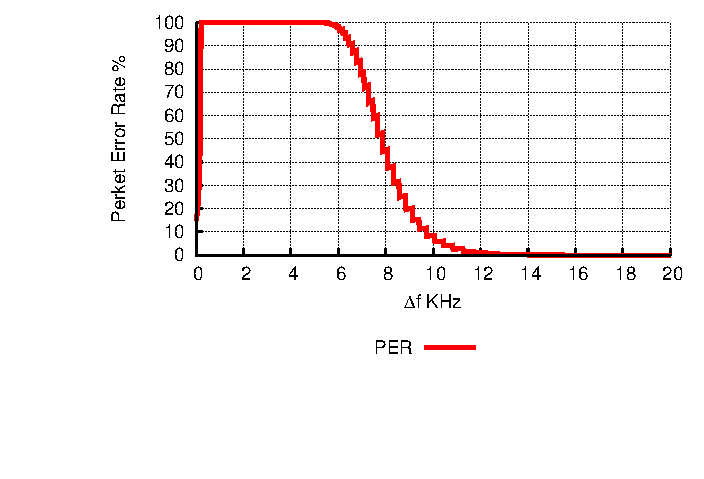
\includegraphics[width=0.45\columnwidth]{envelop_modeling/per_deltaf}
			\label{fig:envelop_modeling_the}
		}
		\subfigure[Simulated Modeling]{
			\includegraphics[width=0.45\columnwidth]{envelop_modeling_sim/per_deltaf_sim}
			\label{fig:envelop_modeling_sim}
		}
	\caption{Figure~\ref{fig:envelop_modeling_the} simulates the PER using equation~\ref{eq:sec:envelop_modeling:per}.
	Whereas the figure~\ref{fig:envelop_modeling_sim} uses 802.15.4 transceiver architectural model. The parameters
	for both plots are: $L = 127$ Bytes, $\alpha = 0.05$, $\Delta f_1 = 0, \Delta f_2$ from 10 to 20 KHz. we can
	find the trend that the PER drops while $\Delta f_2$ increases in both plots. Since the number of consecutive 
	contaminated bits get shorter in larger frequency separation, the possibility for receiver to false decode a
	packet become smaller.}
	\label{fig:envelop_modeling}
\end{figure*}

Figure~\ref{fig:envelop_modeling_the} shows the simulation result of packet error rate (PER) versus
$\Delta f_2$. Parameters of this simulation are: $L = 127$ bytes, $\alpha = 0.05$, $p_{single} = 0.2$
and $\Delta f_2$ from 100 to 20 KHz. Since number of chips $n$, which below threshold $\alpha$ drops
while increasing the frequency. Even number of evnelops $m$ increases but the correct probability 
$p_{correct}$ is close or equal to 1 (if $n$ $<$ chip distance, 13). In contrast, low frequency separation
dramatically deteriorates the $p_{correct}$. The PER is much worse even if the number of envelop $m$ is small.
However, the equations we derived above don't hold under a special case, which is the period of envelop ($T$)
is somehow greater than packet length. Imaging when $m \to \infty$, the PER should be 0 instead of 1. Thus, if the
condition $(1-\gamma)T + (6.5 \mu s(chip distance)/p_{single}) > L\times32 \mu s$ meets, the PER can be written as:
\begin{align}
	PER &= 1 - p_{correct} \\
		&= 1 - \tfrac{(1-\gamma)T - L\times32\mu s + 6.5\mu s/p_{single}}{T - L\times32 \mu s}
\end{align}
Where the $6.5 \mu s/p_{single}$ is the expection value of numbers of error chip, and 
$(1-\gamma)T - L\times32 \mu s + 6.5 \mu s/p_{single}$ is the length for correct decoding. Namely,
if the packet starts within the envelop any moment from 0 $\sim$ numerator, the total error chips is less
than 13 (chip distance). The denominator is the total possible starting point.



\subsection{Architectural Method}
From section~\ref{sec:2tx1rx}, we derived the in-phase and quad-phase signal if the frequency present
in two transmitters and one receiver. We build a complete models of uSDR's transceiver. 
Figure~\ref{fig:envelop_modeling_sim_IQ} shows the received in-phase and quad-phase signal with 
$\Delta f_2 = 15$ KHz. Thus, the period $T$ of envelops is $\tfrac{1}{\Delta f_2} = 66.67 \mu$s. 
\begin{figure}[h]
\centering
	\includegraphics[width=0.98\columnwidth]{envelop_modeling_sim/IQ}
	\caption{This figure shows the received in-phase and quad-phase baseband signals in simulation. The 
	parameters of this simulation are: $\Delta f_1 = 0, \Delta f_2 = 15$ KHz. We can see that the period
	of envelop $T = \tfrac{200 \mu s}{3} = 66.67 \mu s = \tfrac{1}{15 KHz} = \tfrac{1}{\Delta f_2}$}
	\label{fig:envelop_modeling_sim_IQ}
\end{figure}

In the architectural based simulation, we add Gaussian noise to the signal and setting the signal to noise
ration (SNR) to 15dB. In addition to that, we set a threshold, which similar to $\alpha$. If the amplitude
less than $\alpha$, instead of original signal, we randomly generate the noise bounded by $\alpha$. 
From figure~\ref{fig:envelop_modeling_sim}, we can see trend of PER from architectural simulation is similar
to the theoretical method. However, in architectural simulation, the PER never goes to 0 even the $\Delta f$
is large enough. The resaon is the AWGN present and the random noise we added. The random noise wee add not
only exist on low-frequency envelop but the entire signal. Namely, every chip in the sequence is affected by
the noise. Thus, the architectural method has less "effective" chip distance.



\vfill\eject

% page limit          % 14.0 pg

% abstract            % 0.5 pg
\vfill\eject

%\theendnotes

{%\footnotesize
\raggedright
\bibliographystyle{abbrv}
\bibliography{bib}
}

\end{document}

